\documentclass[11pt]{article}
\usepackage{framed, color}
\usepackage{textpos}
\usepackage{natbib}
\usepackage[top=1in, bottom=1in, left=.9in, right=.9in]{geometry}
\usepackage{color}
\usepackage{hyperref}
\usepackage{textcomp}
\usepackage{graphicx}
\usepackage{fancybox}
\usepackage{setspace}
\hypersetup{colorlinks=false, urlcolor=blue, citecolor=black}
\usepackage{soul}
\usepackage{geometry}
\usepackage{color}
\newgeometry{top=1in, bottom=1in, left=.5in, right=.5in}
\usepackage{fancyhdr}
\usepackage{wrapfig}
\usepackage{mdframed}
\pagenumbering{arabic}
\usepackage{fontspec}
\setmainfont{Arial}

\linespread{1.1}

\begin{document}


%\parindent 0.000000001in
\setlength{\parindent}{1cm}
\setcounter{page}{0}
\pagenumbering{arabic}



\fancyhead[CO]{Matthew D. MacManes | Specific Aims}
\pagestyle{fancy}
\setcounter{page}{1}
%\noindent \large{\textbf{\textsc{2. Project:}}}
%\normalsize 
%\begin{center}
%\textsc{{i. Significance}} \\
%\end{center}

The maintenance of water balance is critical for survival. Humans are exquisitely sensitive to changes in osmolality, with slight derangement eliciting physiologic compromise. When the loss of water exceeds dietary intake, dehydration - and in extreme cases, death - can occur. Far from uncommon, millions of people die every year as a direct result of dehydration. In contrast to humans, animals living in desert habitats thrive without water and endure extreme heat and intense drought, as a direct result of unique adaptations. These adaptations allow them to survive conditions fatal to humans and most other animals. Despite being a well-known ecological phenomenon with obvious implications for human health, we know very little of the underlying mechanisms that allow for survival in desert environments. \textbf{The proposed research uses an innovative approach integrating physiology, evolutionary genomics, and computational biology to better understand how animals survive in what appear to be non-survivable conditions.} This proposal represents the foundational steps toward developing the cactus mouse (\textit{Peromyscus eremicus}) as a model system for the study of physiologic water conservation. Indeed, this model offers the scientific community a unique opportunity to gain a deep understanding into the physiology and genomics of osmoregulation in extreme environments – a critically important insight that is impossible using a traditional model system like \textit{Mus}, that like humans, die when subjected to these conditions. While not a part of this proposal, this project lays the groundwork for \ul{\emph{my long-term research goal}} – to identify the causal links between phenotype and genotype, using emerging technologies like the CRISPR-Cas9 system. Ultimately, understanding the mechanisms underlying extreme osmoregulation may suggest novel treatment strategies for conditions (e.g. diarrhea) resulting in acute dehydration in humans.\\

\noindent \textbf{SPECIFIC AIM 1:} To characterize the physiologic and genomic response (differential gene expression, patterns of methylation or isoform use) to extreme water restriction and heat.  

\begin{quote}
The working hypothesis is that while desert-adapted mice may demonstrate genome wide expression patterns suggestive of stress (e.g. activation of HSP, vasopressin responsive pathways) during dehydration, these responses function to preserve normal physiology and thus serum electrolytes will be similar to mice with unrestricted access to water. 

\end{quote}

\noindent \textbf{SPECIFIC AIM 2:} To determine the ontogeny of extreme osmoregulatory ability, from the neonatal period during which fluid (milk) intake is obligate through weaning, when oral fluid intake is exceptionally rare. 

\begin{quote}
The hypothesis here is that patterns of renal gene expression during fetal development through weaning will resemble patterns of gene expression, isoform use, and methylation typical of adult mice when water is freely available. 

\end{quote}

The proposed project aims to integrate studies of physiology, genomics, and computational biology to gain a deep understanding of a fundamental physiological problem – how to conserve water when intake is limited. \ul{\emph{Although dehydration is both common and dangerous, the biology underlying its physiological effects is currently invisible to researchers using traditional mammalian models of disease that lack the eco-evolutionary history present in desert-adapted mice}}. This project will fill a critically important gap in our understanding, which is in support of the specific research aims of the National Institute of Diabetes and Digestive and Kidney Diseases (NIDDK).

\newpage
\fancyhead[CO]{Matthew D. MacManes | Research Strategy}
\pagestyle{fancy}
\setcounter{page}{2}
%\noindent \large{\textbf{\textsc{2. Project:}}}
\normalsize 
\begin{center}
\textsc{{i. Significance}} \\
\end{center}

Dehydration, whether caused by exposure to extreme environmental conditions, water deprivation, or by infection (e.g. diarrheal illnesses) represents a significant threat to human life. In spite of modern medicine, millions of people die every year from dehydration. Compounding issues of exposure and illness, are public health issues regarding the delivery of safe drinking water. With global climate change, these challenges are thought to become only more severe and as a result, \ul{research providing insight into the mechanisms underlying physiologic resistance to acute dehydration is urgently needed.} The response to acute dehydration in humans and traditional mammalian models is generally maladaptive and may include death - this response limits our ability to develop novel insights into this important cause of human mortality. As such, the study of dehydration-tolerant mammalian models will significantly enhance our understanding, and will provide fodder for novel treatments. \textbf{The proposed work aims study extreme osmoregulation in a uniquely suited novel desert-adapted model organism.}

While the mechanisms underlying physiological compromise in dehydration are well characterized \citep{Roberts:2010fl}, some animals possess the ability, much unlike humans, to osmoregulate despite extreme heat and a complete lack of extrinsic water intake \citep{NAGY:1994ta}. Specifically, highly adapted desert mice may never drink water, produce an extremely viscous urine, or no urine at all, and excrete urea in the form of uric acid crystals in the feces \citep{SCHMIDTNIELSEN:1952wi}. This phenotype results in an animal that is very resistant to dehydration-related physiologic compromise, and is in stark contrast to the phenotype of humans and traditional model organisms (e.g. \textit{Mus} and \textit{Rattus}). Although model organisms are attractive targets for study, they lack the requisite biology which may limit insight. In contrast with traditional model organisms, non-model desert-adapted organisms may provide a unique opportunity to study dehydration tolerance, though they typically lack many of the genomic and physiologic tools characteristic of model organisms. Despite this, renal gene expression has been characterized for several genes in desert animals, and was shown to be highly derived in some (e.g. \textit{Dipodomys} \citep{Huang:2001ti}), but not in others (e.g. \textit{Notomys} \cite{Weaver:1994wv}). No studies characterizing genome-wide patterns of gene expression, methylation or isoform use in desert-adapted water stressed animals has been done and therefore the extent to which differences in these parameters underlie phenotype remains unknown. \ul{The proposed work effectively integrates the power of a model organism with the unique biology of a desert-adapted rodent, the cactus mouse (\textit{Peromyscus eremicus}), to generate insights into extreme osmoregulation not current possible.}

\normalsize 
\begin{center}
\textsc{{ii. Innovation}} \\
\end{center}

The proposed work recognizes that successful treatment requires an appropriate model, and while traditional models are powerful, they lack the biology (extreme osmoregulation) upon which more successful interventions may be modeled. The desert-adapted rodent \textit{P. eremicus} retains many of the beneficial characteristics of model organisms, while enhancing opportunity to assay interesting biological phenomenon. In addition to this fundamental innovation, the project it innovative in a number of other ways.
\begin{itemize}
\item Experimental, conceptual, theoretical, and technical innovation: The proposed project leverages unprecedented control over environmental conditions using an ideally suited novel model organism and unique analytical methods to understand the physiologic and genomic response to water deprivation.

\end{itemize}

 

\newpage

\linespread{1.2}

\noindent \textbf{Aim 1:} \ul{To characterize the physiologic and genomic response (differential gene expression, patterns of methylation or isoform use) to extreme water restriction and heat.} \\

To better understand the physiologic and genomic response underlying dehydration resistance, a series of experiments that will allow me to understand how differences in temperature, relative humidity, and water availability affect the desert-adapted rodent \textit{Peromyscus eremicus} will be conducted. These experiments are fundamentally a series of environmental manipulations, described in \hyperlink{Figure 1}{Figure 1}. The experimental design is fully factorial -- meaning that the focal experimental parameter (e.g. water availability) will be tested in the context of the full range of other conditions (e.g. humidity, temperature). Animal care is standardized between experiments and includes measures to reduce the water content of food and bedding materials. Both of these will be dried in a standard desiccation oven to less than 1\% water/volume. Twenty individuals per treatment will be included -- power analyses suggest this sample size will allow for detection of statistical support for patterns with small to medium effect sizes. Together, this design will make it possible to tease-apart the physiologic and genomic response to the various conditions. \\

\vspace{2mm}

\begin{mdframed}
 \begin{center}
  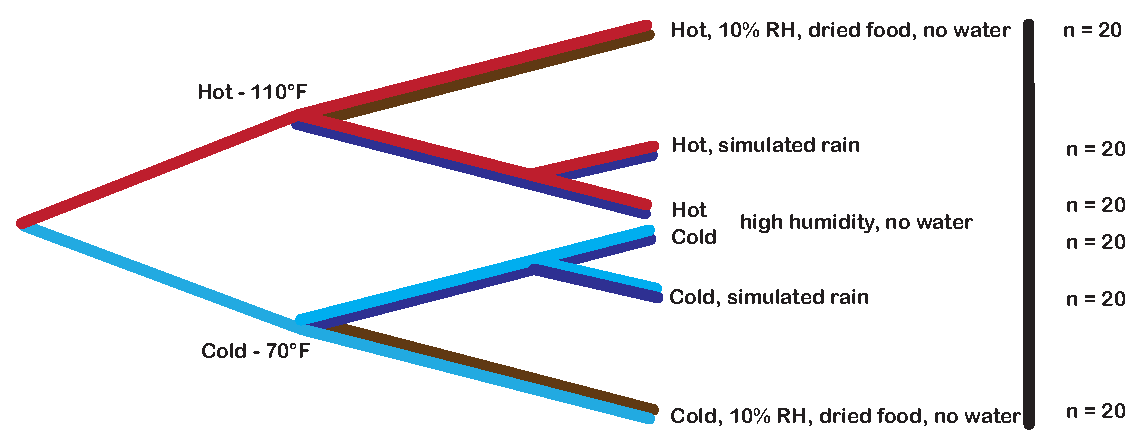
\includegraphics[width=1\textwidth]{exp_design_fig.eps}
 \end{center} 

\noindent \small{Figure 1: Animals are relegated into either hot or cold treatments. Within treatments (n=20 per treatment), animals are exposed to two weeks of varying levels of aridity, from simulated rainfall where water is available \textit{ad libitum}, to dry, where no water is available. RH=relative Humidity}

\end{mdframed}

\vspace{5mm}


For each experiment in Aim 1, physiologic and genomic data will be collected. In the context of limited water intake, how animals achieve electrolyte balance is unknown. Electrolytes are both easy to assay and are critical to physiological well being. Indeed, proper electrolyte balance is fundamental to all other physiological processes like neuronal signal transduction and muscle (including cardiac) contractility. Here, \ul{serum electrolytes} will be measured using the VetScan VS2 critical care panel which includes ALT, BUN, Cl, CRE, GLU, K, Na, bicarbonate ion in a 100uL sample volume. \\

In addition to assaying electrolytes themselves, measures of \ul{urine electrolytes} and \ul{specific gravity} will be collected, as the urinary system represents that major pathway through which these chemicals are lost. These parameters will be measured using an Atago UG-$\alpha$ urine refractometer and tests conducted at the IDEXX reference lab. Lastly, \ul{animals will be weighed} to the nearest 0.1gm every other day, including the day of sacrifice. \ul{Body temperature} will be assayed with weighing using a digital thermometer and probe designed by World Precision Instruments (Sarasota, FL). In connection with this, \ul{feces will be collected} and water content will be assayed using standard methods. \\

Key metabolic parameters such as \ul{carbon dioxide production} and \ul{oxygen consumption} that may influence water consumption will be collected. In addition, the \ul{change in relative humidity} within the metabolic chamber will be assayed, which will allow us to understand the rate of pulmonary water loss (or gain). These tests will be measured during a twenty four hour period at the end of the experimental manipulation, just prior to euthanasia, using a metabolic chamber (Sable Inc.) modified for use in the desert chamber. Together, these data will represent a uniquely rich characterization of the physiological state of a desert rodent held in captivity but importantly, exposed to conditions typical of the natural environment. Of note, all procedures involving vertebrate animals conform to the guidelines provided in \citep{Sikes:2011dz} and have been approved by the University of New Hampshire Animal Care and Use Committee. \\

\noindent \textbf{Aim 1a:} \ul{Determine the physiologic response to drinking-water deprivation, extreme temperature, and humidity in the desert-adapted rodent \textit{P. eremicus}}. I hypothesize that, as a result of unique mechanisms related to solute and water balance, that average serum electrolyte concentrations will remain relatively constant throughout various experimental manipulations, but the variance in measured levels between individuals will increase in the most extreme conditions. These differences will be echoed in differences in urine electrolytes and concentration. Predictions regarding other parameters are detailed in Table 1. \\


Background: The human body consist of 60\% water \citep{Jequier:2009cz}. Far from a static reservoir, proper physiologic function requires water for countless processes including nutrient transport \citep{Haussinger:1996wl}, signal transduction, pH balance, thermal regulation \citep{Montain:1999ux} and the removal of metabolic waste. To accomplish these functions, approximately 2 liters of fluid are used daily - these fluids are lost mainly via the gastrointestinal and genitourinary systems, and by evaporative loss, which is accelerated greatly in extremes of heat and aridity \citep{Cheuvront:2010eg}. These losses must be matched by intake \citep{Jequier:2009cz}, mainly in the form of oral fluid intake. Though the body possesses limited reserves, when loss exceeds intake over even a short period of time, dehydration and in extreme cases, death can occur. Humans and most other animals are exquisitely sensitive to dehydration, and possess limited compensatory mechanisms. In contrast, desert rodents survive in extreme environmental conditions, often without fluid intake. Understanding the mechanisms underlying this remarkable phenotype requires we understand the physiology that accompanies it. The work described here aims to characterize the physiology of dehydration resistance in desert adapted rodents. \\

While the prolonged absence of drinking water is invariably fatal for humans and many other animals, one potentially mitigating effect may be the acquisition of water (or limitation of loss) via the pulmonary vasculature, which is known to be variably permeable to water \citep{Berger:2011ks,Goralski:2010eo}. While pulmonary water acquisition has not been quantified in humans or in mammalian models, the pulmonary vasculature is ideally positioned to retain water from inspired air. Following this, relative humidity -  the amount of extractable water present in respired air may be important to overall hydration status. The design described above incorporates two different levels of humidity to begin to disentangle the effects of drinking water from water acquisition via the pulmonary system. \\
  

Although water stress is obviously important to the survival of desert rodents - a phenotype which is relevant to human health and wellness, extreme temperatures represent another way in which physiological processes may be challenged. While desert animals may thrive in extreme heat, humans cannot. The physiological response is characterized in model organisms, but not in other animals adapted to these conditions. Genes like the heat-shock proteins are protective in humans, but no record of their activity on desert rodents is known. \\

Research Plan:To accomplish this aim, physiologic data from animals held with and without drinking water will be gathered, factorial with respect to the other conditions (e.g. temperature and humidity). The specific experiments described in \hypertarget{Figure 1}{Figure 1} will allow us to tease apart the effects of water deprivation from other parameters. Though the data we propose to collect is described above, in brief, we plan to collect blood and urine electrolytes and urine specific gravity. We will collect data on fecal water content, animal weight and temperature, as well as a battery of metabolic parameters. The specific predictions regarding several of these parameters are described in Table 1.  \\

The statistical treatment of the data will include a multivariate regression (either linear or non-linear) to establish the relationships between the data. Many of these analyses will be conducted with non-parametric tests, as data are often non-normally distributed nor independent. One of the most interesting comparisons will be to understand the relationship between serum sodium and urine sodium, urine concentration, fecal water content, and changes in body weight. Ultimately (e.g. Aim 1b) these data will be linked with patterns of gene expression, methylation, and isoform use to gain a synthetic understanding of dehydration resistance. \\

\vspace{5mm}

%\begin{wrapfigure}{r}[0pt]{1\textwidth}
\hypertarget{Table 1}{}
\vspace{-5mm}
\begin{mdframed}
  \begin{center}
    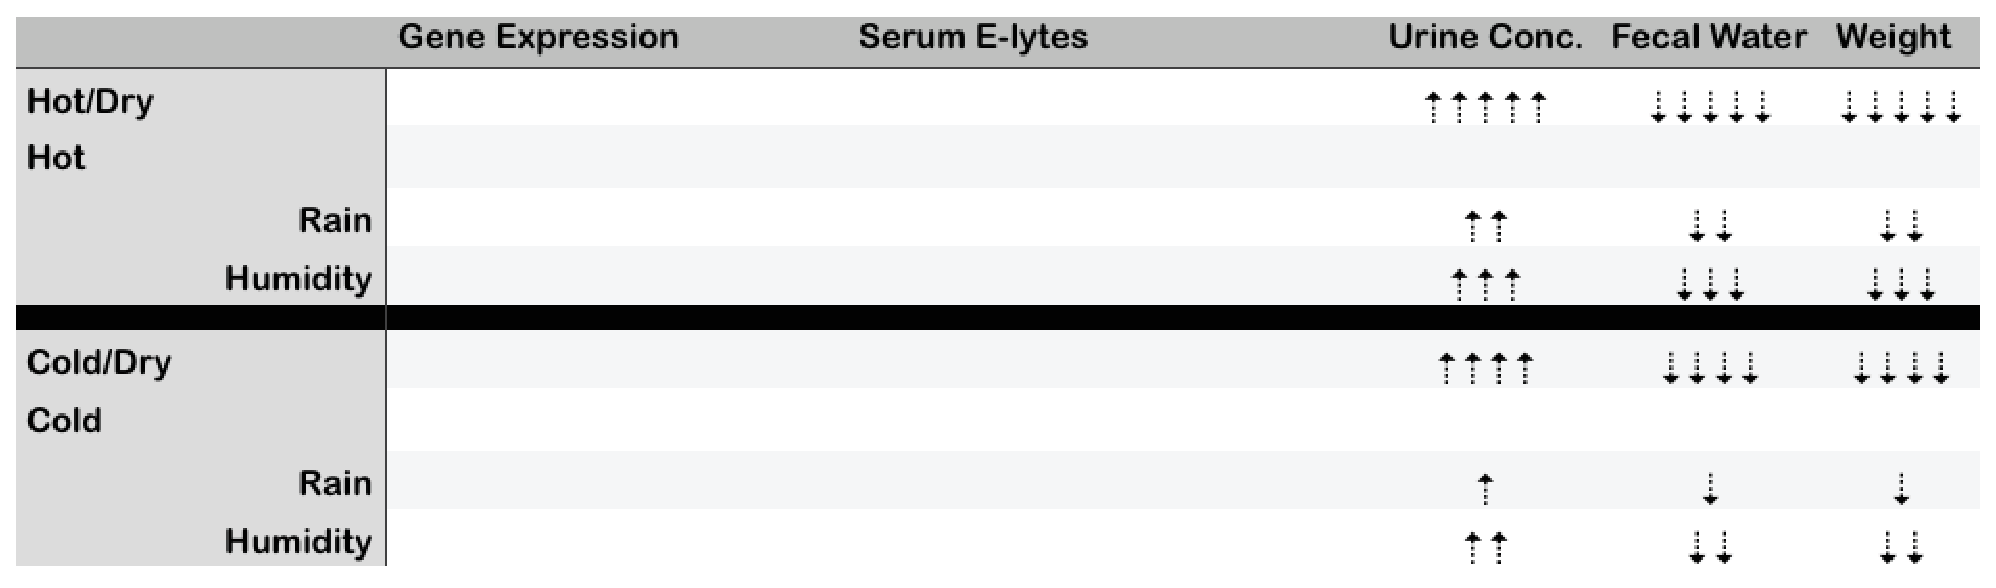
\includegraphics[width=1\textwidth]{Aim1-table.eps}
  \end{center}
  \noindent{\small{Table 1: Say something about predictions here.}}
\end{mdframed}
%\end{wrapfigure}
\vspace{5mm}


% \begin{center}
%  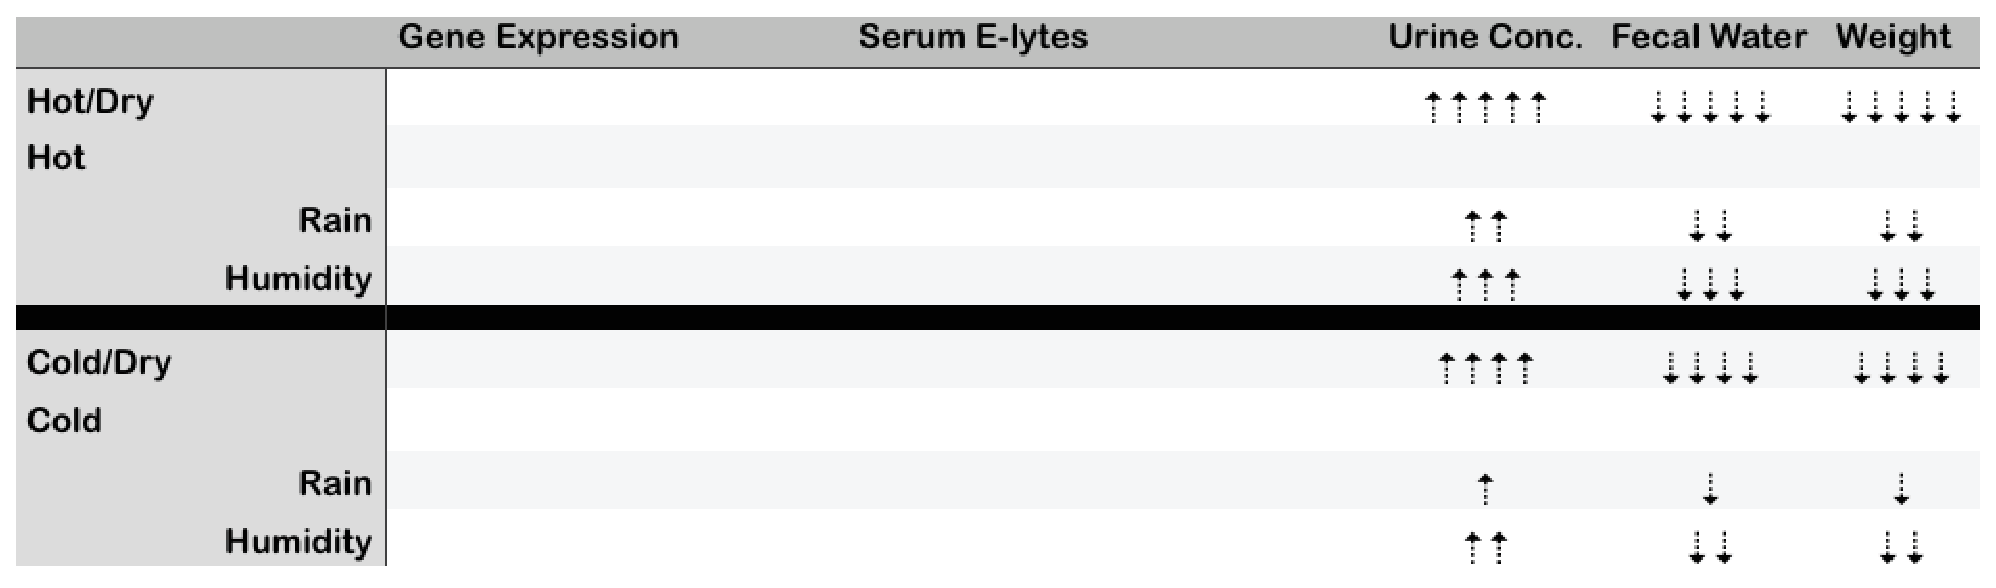
\includegraphics[width=.5\textwidth]{Aim1-table.eps}
% \end{center} 
%
%\noindent \small{Table 1: Say something about predictions here.}
%
%\vspace{4mm}


Preliminary data: I have characterized the electrolyte profile of 2 individuals housed at 70F, 50\% RH, water \textit{ad lib} and two individuals housed in identical conditions except that drinking water was withheld. Despite being housed in typical laboratory conditions, these animals have remarkably unusual electrolyte panel. For instance, mean serum potassium in an un-hemolyzed sample is unusually high at 8.1mg/dL, while Creatinine is low, with a mean measurement of 0.25mg/dL. mean blood urea nitrogen (BUN) is 47mg/dL. In contrast, animals without \textit{ad lib} water were essentially [THIS WILL BE FILLED IN ON FRIDAY] \\  

\noindent \textbf{Aim 1b:} \ul{Define patterns of gene expression, isoform use, and methylation given differences environmental condition}. {I will understand the genetic response to extreme heat and aridity via a series of Illumina bisulfite, Illumina mRNA sequencing, and PacBio mRNA sequencing experiments, and will link these patterns to individual physiologic state as defined in Aim 1.} I hypothesize that genes responsible for water and solute transport will be particularly active in the most extreme conditions in renal and pulmonary tissues, while genes involved in the activation of the hypothalamic-neurohypophysial system will be differentially regulated in the hypothalamus.\\

Background: Broadly speaking, genes underlie the vast majority of observable phenotypes. Whether this relationship is mediated by patterns of expression (e.g. \cite{Teets:2012gt}), which itself may be mediated by differences in methylation \citep{Brenet:2011dq}, or by use alternative splice isoforms \citep{Yukutake:2010ia}, linking genotype to phenotype is extremely difficult. In addition to these mechanisms, function (=phenotype) may be determined by post-translational modifications like phosphorylation of specific sites \citep{Anonymous:2009gb}. The identification of these mechanisms is important, not only because in doing so we gain a deeper understanding of evolution, but also because these molecular mechanisms may be later used as targets for drug development or other therapeutic intervention. With regards to resistance to dehydration, the development of novel therapies is critical, as millions of people die yearly as a consequence. \\

In model organisms, dehydration precipitates a physiological response that is largely driven by the neuroendocrine system. Very much simplified, the cascade begins with the stimulation of osmoreceptors \citep{Arsenijevic:1985bi}, which in turn stimulates neurons located in the paraventricular and supraoptic nuclei of the hypothalamus to release anti-diuretic hormone (ADH) \citep{Zingg:1986vb}. ADH then binds to vasopressin-responsive receptors located in the renal medulla, resulting in aquaporin movement to the surface of the collecting duct \citep{Nielsen:1995uq} which encourages water re-uptake. In addition to the aquaporins, the renin-angiotensin-aldosterone system \citep{Gubler:2010bh}, natriuretic peptides \citep{Totsune:1994kf}, the SLC and mTOR families \citep{Ortells:2012go}, and potentially other yet to be discovered pathways are important to water balance. Far from canonical, each stage in these cascades is dynamic and therefore pathways revealed in \textit{Mus} and humans may not be equivalent to pathways in uniquely adapted desert animals, particularly given radically different phenotypes.\\

The genomic processes related to desert survival have yet to be characterized. The few studies of genetics that have been conducted have focused on the role of expression of single members of the aquaporin gene family (but see \cite{Bartolo:2007hy}), which are large membrane-bound proteins that are critically involved in renal water transport \citep{Kwon:2009bv,Verkman:2002ww,Brown:1995vo,Nielsen:1995cb}. These studies have shown that changes in Aquaporin (AQP) protein abundance and expression may be related to water availability \citep{Boselt:2009fb, Gallardo:2005fm,Bozinovic:2003eg}. In addition to changes in expression, another study showed that the AQP4 pathway was completely lost in the desert rodent \textit{Dipodomys merriami merriami} \citep{Huang:2001ti}. Despite these studies, we have a limited understanding of the genomics of renal water and solute regulation in desert animals. While AQPs are functionally important, water and solute balance is extraordinarily complex, and therefore single-gene studies are necessarily limited in their purview. A more complete understanding of this phenotype and its mechanistic underpinnings will require a sophisticated genome-level approach, which will be the outcome of the proposed research. In contrast to the limited amount known about patterns of renal gene expression, much less is known about gene expression in other tissues, and absolutely nothing about differential methylation or isoform use, even though we know that these complexities are mechanistically important to this specific function \citep{Yukutake:2010ia,Silberstein:2004ex}. \\

Research Plan: The analysis of the genome wide patterns of response to dehydration will be conducted using the same individuals for which I collected physiology data. To accomplish this goal, I will map RNAseq reads derived from kidney, lung, and hypothalamus to the existing annotated draft genome, which was sequenced using startup funds. This phase of the project will be accomplished using the short read aligner BWA \citep{Li:2013wn} and best practices previously established \citep{MacManes:2014io}. Differential expression will be evaluated via the Cufflinks package \citep{Trapnell:2012kp}, while evidence for coordinated changes in large numbers of genes will be detected using the software wcgna \citep{Langfelder:2008bd}. \\

Accurate isoform reconstruction is notoriously difficult using high-throughput short read sequence data such as that produced by Illumina HiSeq platform \citep{Pyrkosz:2013tm,Hiller:2009be}, despite the advent of longer read lengths and newer analytical techniques \citep{LeGault:2013gw,Jiang:2009bw}. In projects like this, where differential isoform use may be critical to phenotype, a different approach may be warranted. For instance, the sequencing technology available from Pacific Biosystems (PacBio) is suggested to provide a resolution to the isoform reconstruction problems \citep{Au:2013hp}, specifically because because it involves a long-read single molecule sequencing strategy \citep{Eid:2009kva}.  To identify patterns of differential isoform use, I will sequence poly-A selected mRNA samples using PacBio technology. Because throughput is relatively low, which may limit the precision with which quantitation can be achieved, I will explore alternative ways to accurately estimate isoform specific expression. One previously unexplored approach involves estimating expression in the program eXpress \citep{Roberts:2012dh} using only those reads that map uniquely and unambiguously to a specific isoform. Because this approach is uncharacterized, I will validate results using a set of isoform specific PCR primers that will allow me to estimate isoform-specific expression using qPCR.   \\ 

Lastly, aside from differences in expression of isoform use, patterns of methylation could be important in the development of extreme osmoregulation - indeed, methylation has been shown to be important to many other complex phenotypes including behavior \citep{Lyko:2010dra}, metabolism \citep{Foret:2012jf}, and physiologic stress (including heat stress) response \citep{Sonna:2002dc}. To understand patterns of methylation, I will generate a large bisulfite sequence dataset, which will contain information from every individual included in the mRNAseq experiments, described above. This dataset will allow for the understanding of another layer of genomic complexity not typically available to researchers conducting RNAseq experiments in isolation. Importantly, in addition to enhancing our understanding of the mechanisms underlying dehydration tolerance, phenotypes related to differential methylation may be prime therapeutic targets.    \\


%\begin{wrapfigure}{l}[0pt]{0.6\textwidth}
%\hypertarget{Table 1}{}
%\vspace{-5mm}
%\begin{mdframed}
%  \begin{center}
%    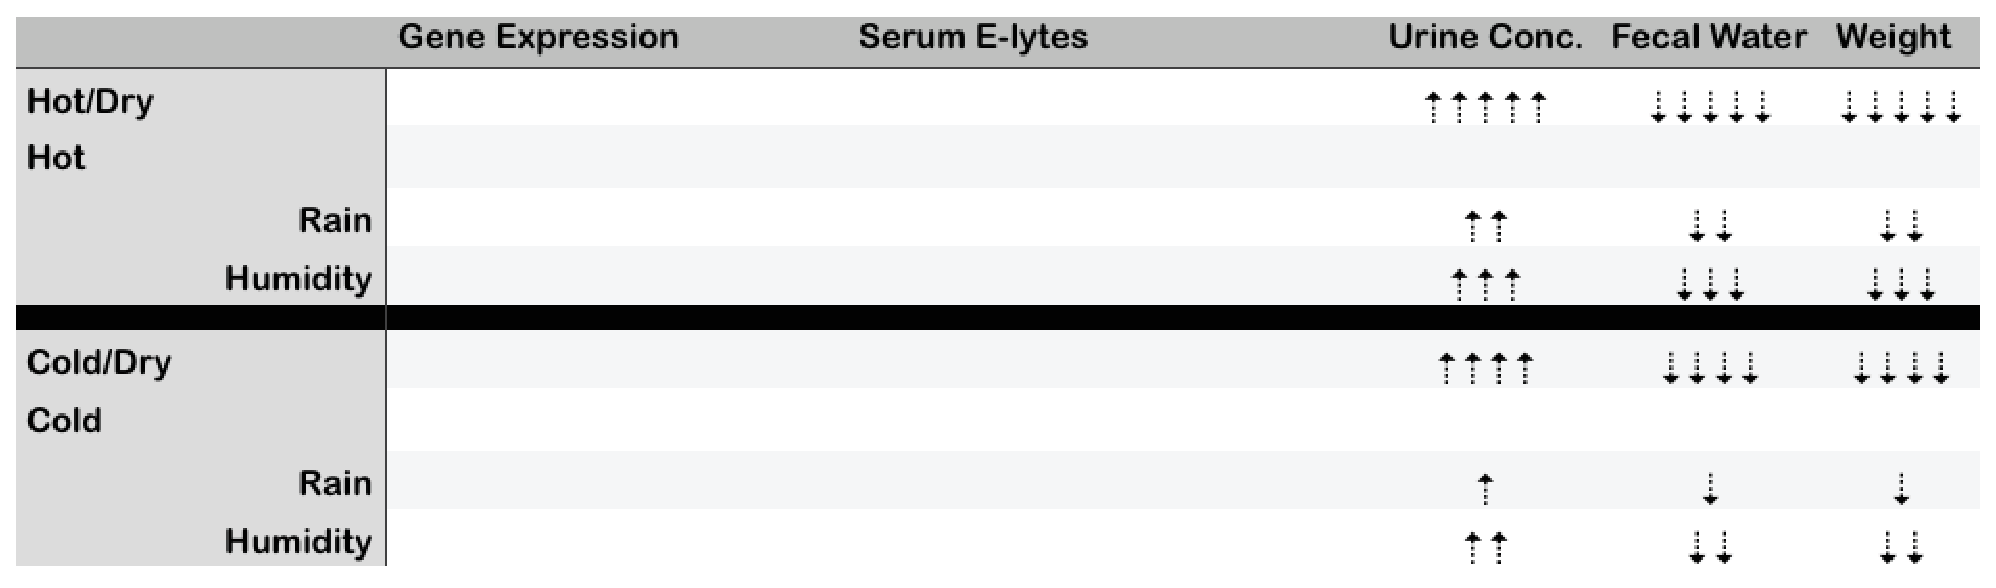
\includegraphics[width=1\textwidth]{Aim1-table.eps}
%  \end{center}
%  \noindent{\small{Table 1: Say something about predictions here.}}
%\end{mdframed}
%\end{wrapfigure}


Preliminary Data: To date, I have generated a RNAseq dataset that consists of approximately 30M 150nt SE Illumina reads from the same 5 animals housed in the 'cold/simulated rain' treatment group from which I collected physiology data. I have [PUT IN RESULTS]. \\

Expected Outcome: Upon completion of Aim 1, I will have a synthetic understanding of the physiologic and genomics patterns associated with extreme osmoregulation. These data will allow me to generate a list of genes, genomic regions, isoforms, and methylation states putatively linked to the phenotype of interest. This list is critical, and will form the basis for my first R01 submission, which will propose the development of a system where manipulation of specific genes is possible (e.g. the CRISPR/CAS9 transgenic system), thus moving the work from correlation to causation. This grant will be developed and submitted during the second year of the COBRE tenure. In addition to this, the completion of Aim 1 will allow me to become more proficient in the collection and bioinformatic analysis of physiology data. Lastly, part of Aim1B involved the development of a novel pipeline for the identification of differential isoform use using PacBio RNA sequence data. This skill will be useful to my broader scientific goals, as well as to the broader scientific community.    \\

Regarding dissemination, the work will be published in open access journals, after rapid release using preprint servers. I envision several papers that are a direct result of this work, include papers describing the physiological and metabolic response to water deprivation as well as their genomic responses. In addition, I aim to publish a more methods-oriented paper surrounding the study of isoform using PacBio data. Aside from peer-reviewed publication, results will be disseminated via social media, my blog, and at the annual meeting of the Society for the Study of Evolution. \\       

%\begin{itemize}
%\item Describe typical renal gene expression profile
%\item link to electrolytes
%\item what I'm going to measure and how
%\item BiSeq, RNAseq, PacBio transcriptome to get at isoforms
%\item expected outcome
%\end{itemize}
%
%
%
%\noindent \textbf{Aim 1c:} Correlate physiology (=phenotype) with genomic patterns. \\
%
%\begin{itemize}
%\item Diff gene expression
%\item coexpression networks
%\item Patterns of isoform use
%\item diff methylation
%\end{itemize}





\noindent \textbf{Aim 2:} \ul{Given the transition from the obligate intake of fluids as infants, to it’s complete absence later in life, the ontogeny of physiologic water conservation will be elucidated.} \\

Background: Given that desert adapted mice, capable of surviving without water are as neonates dependent on liquid intake, {the study of the ontogeny of physiologic water conservation is extremely interesting and relevant to the current work.} The study of individual tissue types samples along the materno-fetal transition in the context of differences in oral fluid intake is remarkably novel and will yield unique insights into physiologic water conservation. \\

Research Plan: This phenomenon will be explored using fetal and neonatal mice whose mothers are exposed to treatments and an abbreviated set of methods listed in Aim 1. Many of the physiological measurements  (e.g. blood and urine analyses) will be impossible to collect in very young animals secondary to sample volume requirements, though a full battery of genomic tests will be possible. To evaluate the ontogeny, five fetal and neonatal mice will be culled per treatment at four different time-points (immediately prior to birth, 2 hours after birth, mid-lactation (approximately 10 days after birth), 1 day after weaning). These time-points have been chosen as together they will allow me to assay the breadth of developmental stages.  I hypothesize that patterns of gene expression, methylation, and isoform use will resemble those common in conditions where water is available \textit{ad lib}, thought the novelty of this aspect of the study limits firm predictions. \\

Expected Outcome: Upon completion of Aim 2, I will have a synthetic understanding of the genomics patterns associated with the ontogeny of extreme osmoregulation. These data, together with the data associated with Aim 1 will allow me to generate a list of genes, genomic regions, isoforms, and methylation states putatively linked to the phenotype of interest. This list is critical, and will form the basis for my first R01 submission, which will propose the development of a system where manipulation of specific genes is possible (e.g. the CRISPR/CAS9 transgenic system), thus moving the work from correlation to causation. This grant will be developed and submitted during the second year of the COBRE tenure.


\begin{center}
\begin{tabular}{l|c c r}

\textsc{Activity} & \textsc{FY2015} & \textsc{FY2016} & \textsc{FY2017} \\
\hline \\
\textsc{Recruit PDF, grad students, undergraduates} & X & & \\
\textsc{Increase Colony Size \& ID animals for experiments } & X & & \\
\textsc{Conduct Physiology Experiments -- AIM 1A} & X & & \\
\textsc{Collect \& Analyze expression data -- AIM 1B} & X & & \\
\textsc{Analyze Bisulfite and PacBio data -- AIM 1B} & & X & \\
\textsc{} & &  &   \\
\textsc{Animal breeding in prep for Aim 2} & & X &  \\
\textsc{Collect \& Analyze genomic data -- AIM 2} & & X & X \\
\textsc{} & &  &   \\
\textsc{Write papers \& submit} & & X & X \\
\textsc{Present results at international conference} & & X & X \\
\textsc{Prepare R01 \& and resubmit as needed} & & X & X \\
\textsc{Train Undergrad, Grad students, \& PDF} & X & X & X \\
\textsc{Disseminate info} & X & X & X \\

\end{tabular}
\end{center}
\vspace{5mm}
\normalsize 
\begin{center}
\textsc{{iii. Relationship to GEBRI program}} \\
\end{center}

%The proposed work has an important synergistic relationship to the larger COBRE proposal. This relationship is founded bioinformatics and genomics, and has an efficient bilevel infrastructure. First the Genome-Enabled Biomedical Research Institute (GEBRI) establishes a set of mentors which will greatly enhance my development as a independent researcher. Specifically Project PI Dr Kelley Thomas provides me with \\


The theme of the proposed COBRE (Genome-Enabled Biomedical Research Institute) focuses on the development genomic resources for novel systems with important relevance to critical issues in human health. Obviously, the work proposed here fits ideally into this theme.  The most important functions for the GEBRI to the long term success of this work include: 

\begin{enumerate}
\item The formation of a collaborative Center bringing together faculty with shared interests in the application of genomics of novel systems, including opportunities to interact with colleagues with and outside UNH.   PI MacManes is already involved in overseeing the weekly genomics group meetings on campus the proposed facilities for this will be exceptional for enhancing that community.

\item The opportunities for mentoring described above represent a valuable resource.  The PI is already participating in the Research Engagement Acadamy and looks forward to participation in the Up-2-NIH program as well as the ongoing mentorship of PIs Thomas and Cote.

\item	Access to high quality genomics and bioinformatics infrastructure and expertise.  PI MacManes brings significant experience and expertise in bioinformatics to the GEBRI. To this end, the MacManes lab has already released a transcriptome assembly pipeline (\url{http://sourceforge.net/projects/tamrs/}) and automated quality control software (\url{http://sourceforge.net/projects/qcpro/}). In addition to this, the PI MacManes is an active developer of the transcriptome assembly program Trinity \citep{Haas:2013jq} and annotation software Trinotate (\url{http://trinotate.sourceforge.net/}). 

\end{enumerate}





%\newpage
%
%\begin{center}
%\textsc{{ii. Background}} \\
%\end{center}
%
%The study of adaptation, or the process through which animals become fitted to their environment has intrigued researchers for decades \citep{Darwin:1859tm, Fisher:1930wy}, though only recently have we had the ability to study the underlying genomic mechanisms. Interestingly, researchers interested in understanding the genetics of adaptation have the ability to ground modern studies of genetics on decades of work aimed at understanding the ecological context within which adaptation occurs. One particularly salient example of the connection between studies of ecology and natural history and modern genomics can be found in the study of physiologic adaptation to desert conditions. Here, remarkable physiologic, morphologic \citep{Dickinson:2007jn,Huntley:1984us,SchmidtNielsen:1950wg,SchmidtNielsen:1952wp} and behavioral \citep{NAGY:1994vd} adaptation has been studied in the context of desert ecology. These studies provide a rich context for the current work, which aims to define the relationship between physiology and genomics in rodents able to thrive in amongst the most harsh of conditions on Earth. 
%
%Though classic research relating morphology (especially renal ultrastructure) and physiology to desert adaptation has been done, we know virtually nothing about how extreme heat and aridity may affect other core physiological and metabolic processes. For instance, the maintenance of normal serum electrolyte concentration is challenging in the context of desert conditions. Indeed, electrolyte derangement is often the ultimate cause dehydration-related death, yet for the vast majority of desert animals, we know nothing of electrolyte balance - not even typical values! Understanding these critical processes is fundamental to our understanding of physiological adaptation, and will be accomplished as part of this project. 
%
%Lastly, 
%
%
%\textbf{Specific Aim 1:}  
%
%\textbf{Specific Aim 2:} 
%
%\textsc{{Preliminary Data:}} . 
%
%\begin{center}
%\textsc{{iv. Broad Impacts}} \\
%\end{center}
%How desert animals survive without water is an intrinsically interesting example of extreme physiology and adaptation. Indeed, telling people of the remarkable story of a rodent that may never drink water is immediately captivating. Having told hundreds of people, including children, adults, scientifically literate and not, the most common response is something like "Wow! That is amazing. How do they do that?" I intend to \textbf{broaden dissemination} by capitalizing on this common response, using traditional and non-traditional methods. While lecture has been the mainstay of scientific communication, its audience tends towards the educated/affluent subset of the population. Given one of my primary goals as a scientists is to broadly share my work, I will use non-traditional modes of communication which will include social media and a blog. All publications are hosted on a public preprint server, and published using using open access options. All data and code is freely available using public repositories like Github, Dryad, or Figshare. In addition to this, I will develop an outreach program that aims to present research findings to school-aged children. These program will be multi-dimensional, with programs geared towards several different age groups. 
%
%\textbf{Broadening participation} is an issue about which I care deeply. As a scientist of Native American descent, I strive to be a role model and mentor for underrepresented groups. To this end, I am developing an internship program- in collaboration with the American Indian Higher Education Consortium (\url{http://aihec.org/}), where qualified Native students may spend a summer working in my lab either in directed or independent research programs. It is my hope that students introduced to my lab via internship may ultimately elect to join the lab. This method of recruitment supplements my general interest in recruiting students from underrepresented groups. 
%
%Lastly, my efforts aimed at broadening dissemination and participation are all within the context of a research program with substantial \textbf{benefits to society}. First, Earth is becoming both warmer and drier, and accurate prediction of animals' response to a changing climate requires knowledge of how animals currently living in dry/hot climates survive - this project will deepen the requisite knowledge. Next, kidney disease effects millions of Americans (\url{http://www.cdc.gov/diabetes/projects/pdfs/ckd_factsheet.pdf}). Though the causes are diverse, the pathophysiology of many resemble dehydration (\textit{e.g.} low renal perfusion pressure). Thus, having a better understanding of how desert rodents endure water stress seemingly without complication may enhance our ability to explain why humans and most other mammals cannot.       
%
%\begin{center}
%\textsc{{v. Summary \& Future Directions}} \\
%\end{center}
%
%The maintenance of water balance in animals is one of the most important physiologic processes, and is critical to survival. Osmoregulation in animals living in desert environments is particularly challenging, as extreme heat and aridity is common. Gaining a deeper understanding of the physiological adaptations that allow for desert survival is important and has obvious implications for climate change science, conservation, and human health and medicine. The proposed research aims to generate a uniquely rich dataset, leveraging cutting edge genomic techniques against careful characterization of physiology, all within an ecological context of desert life. A carefully constructed plan for broadening dissemination and participation ensures that the scientific process as well as its results will be available to all interested parties.  
%
%This proposal represents the foundational steps toward developing \textit{P. eremicus} as a model system for the study of desert adaptation. Indeed, this model offers the scientific community a unique opportunity to gain a deep understanding into the physiology and genomics of desert adaptation- an insight which is impossible to achieve using traditional model system. While not a part of this proposal, this work lays the groundwork for future studies where causal links are made between phenotype and genotype, using technologies like CRISPR-Cas9 and RNAi. 




%\textsc{{Preliminary Data:}} To date, I have generated 40X coverage using a small-insert Illumina dataset and a 3X size selected PacBio dataset using P5-C3 chemistry. I have assembled these reads using a novel approach (in brief, SGA assembly of Illumina data, PacBio reads 'spiked-in' at fm-merge stage). This preliminary assembly strategy has shown promise. A relatively unoptimized process has assembled approximately 2.9Gb of the estimated 3.0Gb genome with a scaffold N50 of 10kb. While still relatively fragmented, we are approaching our short term assembly goal of N50 $\geq$ 25kb.  \\









\newpage
\setcounter{page}{1}
%\thispagestyle{empty}
\singlespacing
\bibliographystyle{model2-names.bst}
\bibliography{formatted.bib}


































\end{document}
